\section{Time-dependent evaluation across checker versions}\label{app:td-evidence}

For a fixed route, all 3 evaluators start from the same materialized arc knots and seek a minimum duration over depot departures. The September 2026 releases prescribe sequences of binary64 operations. The \id{td-binary64-exact-v1} profile specifies the exact minimum on the stored operands and the earliest departure attaining it (Section~\ref{sec:td-core}).

In v0.11.0, \id{td-fold/1} begins with the identity on the departure interval and composes the arc and customer functions in order. Waiting, service and the final depot deadline all use the generic composition routine. In v0.12.0, \id{td-fold/2} restricts the first arc, applies waiting and service directly and cuts the domain at the depot deadline. Its unit-slope shortcut tests equality of the rounded rise and run of an affine segment. Those differences can agree even when the exact slope differs from 1.

Both releases add the route durations in binary64, in order of first customer, and include any fixed vehicle charge. Under \id{td-binary64-exact-v1}, the checker minimizes each route duration on the materialized knots and sums the resulting durations and vehicle charges exactly. Rounding an intermediate time can move it across a jump in the next arc function, as the Rifki-30 route illustrates below.

\subsection{A branch change on the Rifki-30 route}

Consider the customer sequence $\langle23,21,12,3,4,25,30,29\rangle$ from the \href{https://github.com/0nyr/routing-numerical-contracts/blob/75905c8827f959621ea808894e28136d248d2d15/fixtures/rifki30-route.json}{archived Rifki-30 fixture}. Leaving the depot at 1341 puts the vehicle at customer~29 ready to leave at exactly 2880. The return arc has 2 ordinates at that time. Its attained arrival is 3084 and its right-hand limit is 3126 (Figure~\ref{fig:rifki-depot-jump}). The exact duration is therefore $3084-1341=1743$.

\begin{figure}[htbp]
\centering
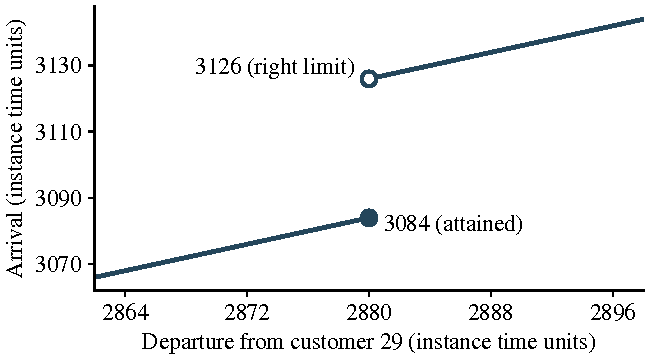
\includegraphics[width=11cm]{figures/rifki30-depot-jump.pdf}
\caption{Final arc $(29,0)$ near departure 2880. The filled point gives the arrival at the knot. Moving one binary64 step to its right crosses the jump, although that horizontal displacement is too small to see at this scale.}\label{fig:rifki-depot-jump}
\end{figure}

At initial departure 1341, v0.11 computes the ready time as \id{2880.0000000000005} and takes the upper branch. Its minimum over all departures is 1768 at 1301. Both v0.12 and the exact reference give 1743 at 1341. The jump of 42 at one arc thus changes the optimized route duration by 25.

\FloatBarrier
\subsection{Agreement on archived routes}

Of 3,072 TD incumbent records in the frozen store, 3,052 had the files needed to materialize their arc functions. Re-evaluating those same route sets under the two releases changed 871 solution objectives, with a largest absolute change of 25 in the corresponding instance's units. The two releases gave the same temporal-feasibility verdict on every available route set.

We compare both releases with the exact reference on 146 published Lera-Romero solutions on Dabia2013 instances and 35 stored solutions selected across families, problem types and sizes up to 100 customers. In Table~\ref{tab:td-release-agreement}, a match means agreement with the exact value rounded once to binary64. For a complete solution we sum the exact route durations and add any fleet charge before rounding. For a departure we run the exact forward schedule at the binary64 time returned by the released fold.

\begin{table}[htbp]
\centering
\small
\begin{tabular}{@{}lrrrr@{}}
\toprule
& \multicolumn{2}{c}{Dabia2013} & \multicolumn{2}{c}{Broader panel}\\
\cmidrule(lr){2-3}\cmidrule(l){4-5}
Comparison & v0.11 & v0.12 & v0.11 & v0.12\\
\midrule
Route duration matches & 455/898 & 494/898 & 151/243 & 175/243\\
Reported departure infeasible & 148/898 & 140/898 & 14/243 & 11/243\\
Solution objective matches & 70/146 & 70/146 & 14/35 & 28/35\\
\bottomrule
\end{tabular}
\caption{Released folds compared with exact evaluation on identical inputs. Every listed route has an exact feasible departure. The middle row tests the particular departure returned by each fold.}\label{tab:td-release-agreement}
\end{table}

On Dabia2013, v0.12 matches 39 more route durations, yet both releases match the rounded exact total on 70 solutions. On the broader panel v0.12 matches twice as many solution totals as v0.11. A rounded match establishes agreement at display precision. The \href{https://github.com/0nyr/routing-numerical-contracts/tree/75905c8827f959621ea808894e28136d248d2d15/results}{frozen results} identify the input, routes and release outputs for each comparison.

\subsection{Time to evaluate one route}

We use the archived serial measurements on an Intel i7-12700H with CPython 3.13.13. Within each panel a fixed hash ordering selected 12 routes with at most 25 customers. Table~\ref{tab:td-matched-runtime} compares all 3 implementations on those same routes. Both released folds start with the arc functions in memory. For the exact profile we time the study's independent reference. It constructs the rational functions for the route, partitions the departure interval at preimages of their boundaries and minimizes duration over that partition.

\begin{table}[htbp]
\centering
\small
\begin{tabular}{@{}lrrrr@{}}
\toprule
Panel & Routes & v0.11 fold (ms) & v0.12 fold (ms) & Exact reference (ms)\\
\midrule
Dabia2013 & 12 & 0.083 & 0.053 & 17.228\\
Broader panel & 12 & 0.302 & 0.218 & 102.475\\
Combined & 24 & 0.121 & 0.066 & 36.910\\
\bottomrule
\end{tabular}
\caption{Median milliseconds per route. For each route we first take the median of 7 calibrated batches per released fold or 3 complete calls to the exact reference. Each route has equal weight in the panel median.}\label{tab:td-matched-runtime}
\end{table}

Taking the time ratio separately for each route gives a median exact-reference time of $315.2$ times the v0.11 fold time and $482.9$ times the v0.12 fold time. These ratios include the reference's construction of rational stages and its partitioning algorithm. They measure the present cost of independently checking a route on this panel. The native study below measures complete fixed-solution checks, and the Kayros pilot examines the additional work of proving an optimum. A solver can use a fast fold to propose routes and submit them for exact evaluation. Proving optimality under the new profile also requires bounds valid for that profile. The \href{https://github.com/0nyr/routing-numerical-contracts/blob/75905c8827f959621ea808894e28136d248d2d15/results/controlled-td.json}{individual calls and fold timings} are available for reproducing the comparison.

\subsection{Two exact algorithms for certifying a submitted solution}\label{app:td-native}

A fast exact checker can exploit the fact that each vehicle clock is nondecreasing. We compare 2 algorithms on the same binary64 operands. Both convert each operand to its exact rational value, use inclusive deadlines and return the minimum duration and the earliest departure attaining it. The C++ implementations share the same GMP rational knots, interval slopes and Python binding. The \href{https://gmplib.org/manual/Rational-Conversions}{GMP conversion from binary64} is exact.

\paragraph{Compose the route prefix.}
After each visit, keep the arrival or ready time as a piecewise-affine function of the initial departure. To append an arc, scan the prefix and arc knots in time order. Where an increasing prefix segment crosses an arc knot, insert its exact preimage into the new prefix. At a jump, keep the attained ordinate and the right limit separately. If the prefix stays constant at an arc knot, the vehicle attains the lower ordinate throughout that plateau. Waiting can add a breakpoint, and a deadline can truncate the feasible interval. Finally compare return time minus departure at the attained breakpoints in increasing departure order. For continuous FIFO functions, Visser and Spliet give a linear-time scan for each composition. Here the scan also carries the two ordinates at a jump. \href{https://repub.eur.nl/pub/100852/EI2017-23.pdf}{Visser and Spliet, Section~3}.

\paragraph{Sweep through departures.}
Evaluate the lowest allowed departure first. If it is infeasible, FIFO and the closed upper bounds exclude all later departures. Otherwise trace the vehicle's clock through the route. Just to the right of that departure, the clock at each visit has an exact value and rate of increase. A positive rate determines when it will next meet an arc knot, waiting threshold or deadline. A zero rate at a knot keeps the vehicle on its attained branch. The first event across the visits ends an interval on which route duration is affine. Left continuity gives the attained return at its right endpoint. Repeating this operation visits the candidates for the minimum without constructing every prefix function. Both algorithms test singleton domains and keep the earliest departure on a tie.

\begin{table}[htbp]
\centering
\small
\begin{tabular}{@{}lrr@{}}
\toprule
Evaluator & Including preparation (ms) & Prepared (ms)\\
\midrule
Python exact partitioning reference & 30.217 & \\
Python exact departure sweep & 1.794 & 1.065\\
C++/GMP exact prefix composition & 0.234 & 0.134\\
C++/GMP exact departure sweep & 0.236 & 0.125\\
Python v0.12 released fold & & 0.063\\
\bottomrule
\end{tabular}
\caption{Grid'5000 timings on the same 24 routes as Table~\ref{tab:td-matched-runtime}. Entries are median milliseconds per route. Blank cells indicate unmeasured scopes. The released fold returns its historical binary64 result.}\label{tab:td-native-route}
\end{table}

We ran 2 fresh serial processes on the Nancy Grid'5000 cluster, pinned to 1 logical CPU of a Xeon Gold 5220, using CPython 3.13.12, GCC 14.2 and GMP 6.3. For each route and method, each process warms the call and times 3 calibrated batches. We take the median within each process, then the median across processes, then across routes. In the preparation-inclusive scope the new algorithms start with the binary64 operands gathered for the route. The original partitioning reference also rebuilds its arc lookup from the loaded record. In the prepared scope the arc representations are already in memory. Both native scopes include transferring the exact result to Python. The median paired speedup over the partitioning reference is $107.3$ for native composition including preparation. On the Grid'5000 node, prepared native composition takes $1.84$ times the v0.12 route time by the same paired comparison. Repeating the matched comparison on an i7-12700H gave a median paired speedup of $144.6$ for preparation-inclusive native composition over the Python partitioning reference.

For a submitted solution the checker starts with the instance fields and an index of its materialized binary64 arcs. It checks route coverage, fleet size and capacities, gathers and prepares each route, optimizes its departure and sums the exact durations and any vehicle charge. File loading, family materialization and result serialization are outside this timer. Both native algorithms reproduce the independent partitioning reference's exact durations and earliest departures for all 1,141 routes. The resulting median time for a complete solution is 1.36~ms for composition and 1.35~ms for the sweep on the 146 Dabia2013 solutions. On the 35 broader solutions the medians are 18.35~ms for composition and 14.26~ms for the sweep (Figure~\ref{fig:td-native-solution}).

\begin{figure}[htbp]
\centering
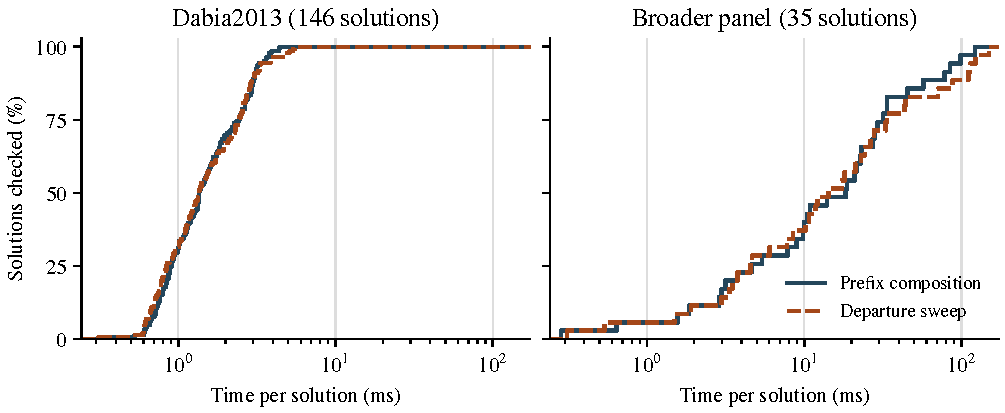
\includegraphics[width=0.92\linewidth]{figures/td-fixed-solution-time.pdf}
\caption{Fraction of submitted solutions checked within a given time, including route preparation, exact scheduling and objective aggregation. Each point is the median for one instance and candidate. The horizontal scale is logarithmic. Times are from the Grid'5000 node.}\label{fig:td-native-solution}
\end{figure}

In a separate scale check on the i7-12700H we selected one available solution per family at its largest available customer count, resolving ties by record identifier. On the 2 selected 1,000-customer solutions, native composition checked 91 Lera2026 routes in 79~ms and 66 Poryos2026 routes in 465~ms. The departure sweep took 89 and 779~ms respectively. These cases illustrate the effect of route structure and arc complexity at the same customer count.

\paragraph{Starting from an instance file.}
We timed the released v0.12 loader followed by the native composition checker on 3 published route sets. These cases exercise a stored ATF, reconstruction from a road graph and traffic overlay, and reconstruction from an IGP speed profile. The loader reads the descriptor and candidate and verifies the materialized ATF identity. The checker builds its model, validates the solution and computes the exact objective and departures. The last step writes the exact result to a JSON buffer. Each case ran in 5 fresh processes on the Grid'5000 node with a warm filesystem cache. We verified the result with the departure sweep after each run.

\begin{table}[htbp]
\centering
\small
\begin{tabular}{@{}lrrrr@{}}
\toprule
Instance & Customers & Load (ms) & Check (ms) & Total (ms)\\
\midrule
Blauth-Nairobi, stored & 10 & 3.02 & 0.67 & 3.98\\
Poryos-Lyon, road graph & 10 & 437.59 & 3.74 & 441.95\\
Lera C1\_2\_1 S1, IGP & 200 & 926.08 & 26.62 & 953.24\\
\bottomrule
\end{tabular}
\caption{Median times from input files to a serialized exact result using the released loader and prototype checker. Each column is a separate median. The total includes result serialization.}\label{tab:td-native-loader}
\end{table}

For the 200-customer Lera case the loader reconstructs and verifies 40,200 directed ATFs before checking the submitted routes. For repeated submissions to the same instance, retaining the verified materialization in memory can therefore save more time than changing the route algorithm.

\paragraph{What exact solution records have to store.}
Both native algorithms agreed on feasibility, duration and earliest departure for all 61,500 routes on the 3,052 available incumbent records. An independent exact forward traversal replayed every departure and recovered all route durations and solution objectives. The 20 records with unavailable materialization files remain outside this comparison. The released solution total matched the once-rounded exact objective on 1,300 records under v0.11 and 1,565 under v0.12. Equality of the released value with the unrounded rational objective held on 454 and 624 records, respectively.

Even when every stored operand is binary64, TD interpolation and boundary preimages can introduce non-dyadic denominators. Summing routes can give a much longer denominator than any individual route requires. Across the store, the largest integer in an exact route duration or departure had 1,093 decimal digits. For 358 solution totals, the reduced numerator or denominator exceeded 4,300 digits, the \href{https://docs.python.org/3.13/library/stdtypes.html#integer-string-conversion-length-limitation}{default threshold for ordinary decimal integer conversions in CPython}. One 1,000-customer Poryos-Lyon solution had a numerator of 10,405 digits. An implementation of Section~\ref{sec:results} must preserve every digit of these strings. All 3,052 exact objectives round-tripped as canonical decimal strings on the Grid'5000 node. The largest numerator and denominator together occupied 20,837 bytes in their compact JSON record. This encoding test is separate from scheduling.

\FloatBarrier
\subsection{From a checked route to an optimality proof in Kayros}\label{app:td-kayros}

Checking a submitted solution supplies an exact upper bound. To measure the additional work needed for a lower bound, we took 2 complete 10-customer Rifki2020 instances, ran the Kayros 1.8 repair checkout using its historical \id{td-fold/1} objective, and solved the same instances independently under \id{td-binary64-exact-v1}. We used every directed arc and every capacity-admissible customer order. Rifki-1 was the first numbered instance. We selected Rifki-13 because a previous pricing audit had identified a discrepancy on one of its routes.

\begin{table}[htbp]
\centering
\small
\begin{tabular}{@{}lrr@{}}
\toprule
 & Rifki-1 & Rifki-13\\
\midrule
Capacity-admissible route orders & 7,396 & 37,180\\
Temporally feasible route orders & 4,527 & 37,180\\
Exact optimal solution duration & 3,594 & 4,128\\
\midrule
Kayros branch-and-price, historical fold (s) & 0.384 & 6.257\\
Enumeration with integral breakpoints (s) & 0.479 & 5.919\\
Enumeration with general GMP composition (s) & 5.769 & 70.680\\
\bottomrule
\end{tabular}
\caption{Whole-instance wall times, including input loading, on the same Grid'5000 CPU as Table~\ref{tab:td-native-route}. The first 2 time rows give medians of 3 fresh processes. The last gives 1 run per instance. The enumeration times include the subset dynamic program that selects the best collection of routes.}\label{tab:td-kayros-pilot}
\end{table}

On these 2 instances, all knot coordinates, service times and window bounds are integers and all affine arc slopes are 0 or 1. Each affine prefix therefore has slope 0 or 1 and integer intercept. An increasing prefix reaches an integer threshold at an integer departure. By induction all cuts of the feasible route profile are integral, including an earliest minimizer. This justifies testing integer departures on these instances under the continuous-time rule. The specialized implementation shares prefix computations and evaluates the eligible integer times in batches. General GMP composition instead solves each admissible ordered route independently over continuous time. The two methods agree on feasibility for all 44,576 orders and on the exact duration and earliest departure of every feasible order.

Kayros returned routes attaining the exact optimum on both instances. Its fold gave a total of \id{4127.999999999996} on Rifki-13. A different route, $\langle4,9,5,8,6\rangle$, exposes a larger discrepancy. Its historical minimum was 2372 at departure 2146, and the exact minimum is 2370 at 1440. An exact check of the returned solution alone would not reveal that change to a competing column.

We also obtained a lower bound from the set-partitioning relaxation over the complete route list. On Rifki-1, exact verification of a primal and a dual solution gives 3594 at the root. On Rifki-13 the root relaxation gives $16167/4=4041.75$. Adding the 120 three-customer subset-row inequalities raises the verified bound to 4128. For each triple, at most one route in an exact cover can visit two or more of its customers. In both certificates we checked exact primal feasibility, dual signs, equality of objectives and nonnegative reduced cost on every feasible route. These certificates were obtained independently of the Kayros pricing engine.

\paragraph{Do the multipliers used by Kayros certify its root?}
We recorded the final LP multipliers, active cuts and forbidden arcs in a separate run of the same solver on each instance. Both searches ended at the unrestricted root. At Rifki-1 the stored multipliers already give a lower bound of 3594. The minimum exact reduced cost across all 4,527 feasible routes is zero.

At Rifki-13, Kayros used 12 subset-row cuts. With its binary64 multipliers read exactly, 3 of the 37,180 feasible routes have negative reduced cost. Route $\langle 1,7\rangle$ attains the smallest value, $-2^{-43}$. The multipliers are all close to integers. We used their nearest integers as a candidate dual, verified the signs of the cut multipliers and checked every route inequality against the exact route duration. The minimum reduced cost is then zero and the verified dual objective is exactly 4128. Since the submitted routes attain 4128, this proves optimality directly. Rounding serves only to propose a dual witness. Its validity follows from checking all inequalities, a test that can also reject the proposed witness.

Starting from the saved complete route catalog, solver result and trace, the independent verifier took 0.118~s on Rifki-1 and 0.676~s on Rifki-13 (medians of 3 fresh processes). These times include reading the files and checking the duals. Constructing the catalogs takes the separate enumeration times in Table~\ref{tab:td-kayros-pilot}, which also include selecting an optimum. A production Kayros integration must establish a lower bound over every permitted route at a closing node, including routes discarded during pricing. Both pilot instances close at the root. A branching instance with nonintegral route costs would test pricing, dominance and node pruning under the proposed profile.

